\documentclass{article}
\usepackage[a4paper, left=1mm, right=1mm, top=5mm, bottom=5mm]{geometry}
\usepackage[pdftex]{graphicx}
\usepackage{ucs}
\usepackage{tikz}
\usepackage{pgfplots}
\pgfplotsset{compat=1.9}
\usepackage{pgfplots}
\usepackage[utf8x]{inputenc} % Включаем поддержку UTF8  
\usepackage[russian]{babel}  % Включаем пакет для поддержки русского языка 
\graphicspath{{/}}
\linespread{2}
\DeclareGraphicsExtensions{.jpg}
\begin{document}

\includegraphics[width=2.4cm]{mirea} 
\begin{center}
\begin{LARGE}
\textbf{Московский государственный технический университет}\\
\textbf{радиотехники, электроники и автоматики}\\
\textbf{(МГТУ МИРЭА)} \\
~\\
\hrule \vspace {10pt}
\textbf{Институт высоких технологий} \\

\textbf{Кафедра «Теплофизические приборы и аппараты»} \\
Дисциплина (модуль) \textbf{«Информационные технологии\\
в АКТ»} \\
\end{LARGE}
\begin{Huge}
\textbf{Домашняя Работа}\\
\end{Huge}
\begin{large}
Тема: 
\end{large}
\begin{normalsize}
“Расчет параметров двигателя на квазистационарных режимах” \\
\end{normalsize}
~\\
~\\
\begin{large}
Вариант №14\\

\end{large}
\end{center}
\begin{flushright}
Выполнил студент группы ВТ7 - 1201\\
\rule{4cm}{0.01pt} / А.Л. Чукаева / \\
~\\
\end{flushright}
\begin{flushleft}
Отметка о защите \rule{5cm}{0.01pt} \\
\end{flushleft}
\begin{flushright}

Преподаватель каф. ВТ-7 \\
\rule{4cm}{0.01pt} / В.В. Кадомкин / \\
~\\
~\\
\end{flushright}
\begin{center}
\textbf{Москва - 2015}
\end{center}

\begin{flushright}
\begin{scriptsize}
\textit{160700.65   Проектирование авиационных и ракетных двигателей\\
 Информационные технологии в АКТ: Лабораторный практикум} \\
\end{scriptsize}
\end{flushright}

\begin{center}
\begin{large}
\textbf{\textit { Building a profile nozzle }} \\
\end{large}
\end{center}

\begin{center}
\begin{tiny}
\begin{tabular}{|l*{16}{l|}}
\hline
i & li & \(D_i\) & \(F_i\) & \(F_{kr}/F_i\) & $\lambda_i$ & q($\lambda_i$) & $\pi(\lambda_i$) & $\tau(\lambda_i$) & $\varepsilon(\lambda_i$) & q($\lambda_i) - F_{kr}/F_i$ & P & T & \(R_0\) & v  \\
\hline
-5 & -0.059703 & 0.500000 & 0.196344 & 0.011825 & 0.007358 & 0.011825 & 0.999970 & 0.999995 & 0.999976 & -0.000000 & 13999583 & 3199.982829 & 17.891072 & 6.824127 \\
-4 & -0.047762 & 0.410874 & 0.132585 & 0.017511 & 0.010897 & 0.017511 & 0.999935 & 0.999988 & 0.999947 & -0.000000 & 13999086 & 3199.962341 & 17.890551 & 10.106071 \\
-3 & -0.035822 & 0.321748 & 0.081304 & 0.028556 & 0.017772 & 0.028556 & 0.999826 & 0.999969 & 0.999858 & -0.000000 & 13997570 & 3199.899835 & 17.888963 & 16.481898 \\
-2 & -0.023881 & 0.232623 & 0.042499 & 0.054630 & 0.034013 & 0.054630 & 0.999364 & 0.999885 & 0.999479 & 0.000000 & 13991101 & 3199.633135 & 17.882187 & 31.542967 \\
-1 & -0.011941 & 0.143497 & 0.016172 & 0.143565 & 0.089662 & 0.143565 & 0.995590 & 0.999203 & 0.996384 & -0.000000 & 13938259 & 3197.450600 & 17.826809 & 83.151114 \\
0 & 0.000000 & 0.054371 & 0.002322 & 1.000000 & 0.999700 & 1.000000 & 0.560819 & 0.900960 & 0.622468 & -0.000000 & 7851461 & 2883.073201 & 11.136885 & 927.104324 \\
1 & 0.023030 & 0.071136 & 0.003974 & 0.584198 & 0.389441 & 0.584198 & 0.919450 & 0.984970 & 0.933480 & 0.000000 & 12872297 & 3151.904598 & 16.701362 & 361.161046 \\
2 & 0.046060 & 0.087900 & 0.006068 & 0.382608 & 0.244614 & 0.382608 & 0.967557 & 0.994070 & 0.973329 & 0.000000 & 13545800 & 3181.024962 & 17.414319 & 226.850874 \\
3 & 0.069091 & 0.104665 & 0.008604 & 0.269856 & 0.170133 & 0.269856 & 0.984196 & 0.997132 & 0.987028 & -0.000000 & 13778749 & 3190.820918 & 17.659414 & 157.778838 \\
4 & 0.092121 & 0.121429 & 0.011580 & 0.200487 & 0.125650 & 0.200487 & 0.991355 & 0.998435 & 0.992908 & -0.000000 & 13878963 & 3194.993353 & 17.764621 & 116.525939 \\
5 & 0.115151 & 0.138194 & 0.014999 & 0.154795 & 0.096733 & 0.154794 & 0.994869 & 0.999073 & 0.995792 & -0.000000 & 13928160 & 3197.032668 & 17.816220 & 89.708209 \\
6 & 0.138181 & 0.154959 & 0.018859 & 0.123113 & 0.076815 & 0.123113 & 0.996762 & 0.999415 & 0.997345 & -0.000000 & 13954663 & 3198.128859 & 17.844004 & 71.236464 \\
7 & 0.161211 & 0.171723 & 0.023160 & 0.100248 & 0.062492 & 0.100248 & 0.997856 & 0.999613 & 0.998242 & -0.000000 & 13969980 & 3198.761568 & 17.860056 & 57.954241 \\
8 & 0.184241 & 0.188488 & 0.027903 & 0.083208 & 0.051842 & 0.083209 & 0.998524 & 0.999734 & 0.998790 & 0.000000 & 13979335 & 3199.147725 & 17.869859 & 48.077187 \\
9 & 0.207272 & 0.205252 & 0.033087 & 0.070171 & 0.043704 & 0.070171 & 0.998951 & 0.999811 & 0.999140 & 0.000000 & 13985311 & 3199.394303 & 17.876120 & 40.530025 \\
10 & 0.230302 & 0.222017 & 0.038712 & 0.059974 & 0.037344 & 0.059974 & 0.999234 & 0.999862 & 0.999372 & -0.000000 & 13989273 & 3199.557758 & 17.880272 & 34.632107 \\
11 & 0.253332 & 0.238782 & 0.044779 & 0.051848 & 0.032279 & 0.051848 & 0.999428 & 0.999897 & 0.999531 & -0.000000 & 13991985 & 3199.669582 & 17.883113 & 29.935098 \\
12 & 0.276362 & 0.255546 & 0.051288 & 0.045268 & 0.028180 & 0.045268 & 0.999564 & 0.999921 & 0.999642 & -0.000000 & 13993891 & 3199.748179 & 17.885109 & 26.133349 \\
13 & 0.299392 & 0.272311 & 0.058238 & 0.039866 & 0.024815 & 0.039866 & 0.999662 & 0.999939 & 0.999723 & 0.000000 & 13995263 & 3199.804726 & 17.886546 & 23.012874 \\
14 & 0.322423 & 0.289075 & 0.065630 & 0.035376 & 0.022019 & 0.035376 & 0.999734 & 0.999952 & 0.999782 & 0.000000 & 13996270 & 3199.846253 & 17.887601 & 20.419854 \\
15 & 0.345453 & 0.305840 & 0.073462 & 0.031604 & 0.019670 & 0.031604 & 0.999787 & 0.999962 & 0.999826 & 0.000000 & 13997023 & 3199.877302 & 17.888390 & 18.241776 \\
\hline
\end{tabular}

\end{tiny}
\end{center}

\begin{flushright}
\textit{ Table $N^o 5$: Data table to build the profile of the nozzle } \\
\end{flushright}
\begin{tikzpicture}

\begin{axis} [
legend pos = outer north east,
height = 0.19\paperheight,
width = 0.4\paperwidth ]
\legend{  P };
\node[anchor=south west,inner sep=0] at (0,0) {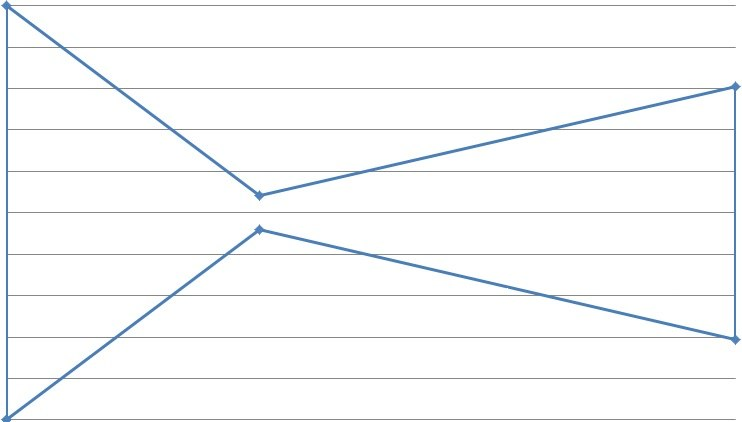
\includegraphics[width=5.7cm, height=3.4cm]{fon.jpg}};
\addplot[mark = none,line width = 0.05 cm, draw =  red ] coordinates {
( -0.059703 , 13999583.000000 )
( -0.047762 , 13999086.000000 )
( -0.035822 , 13997570.000000 )
( -0.023881 , 13991101.000000 )
( -0.011941 , 13938259.000000 )
( 0.000000 , 7851461.000000 )
( 0.023030 , 12872297.000000 )
( 0.046060 , 13545800.000000 )
( 0.069091 , 13778749.000000 )
( 0.092121 , 13878963.000000 )
( 0.115151 , 13928160.000000 )
( 0.138181 , 13954663.000000 )
( 0.161211 , 13969980.000000 )
( 0.184241 , 13979335.000000 )
( 0.207272 , 13985311.000000 )
( 0.230302 , 13989273.000000 )
( 0.253332 , 13991985.000000 )
( 0.276362 , 13993891.000000 )
( 0.299392 , 13995263.000000 )
( 0.322423 , 13996270.000000 )
( 0.345453 , 13997023.000000 )
};
\end{axis}
\end{tikzpicture}
\begin{flushright}
\textit{ Pic. $N^o 14$: Schedule changes in pressure on the projected profile of the nozzle } \\
\end{flushright}
\begin{tikzpicture}
\begin{axis} [
legend pos = outer north east,
height = 0.19\paperheight,
width = 0.4\paperwidth ]
\legend{  T };
\node[anchor=south west,inner sep=0] at (0,0) {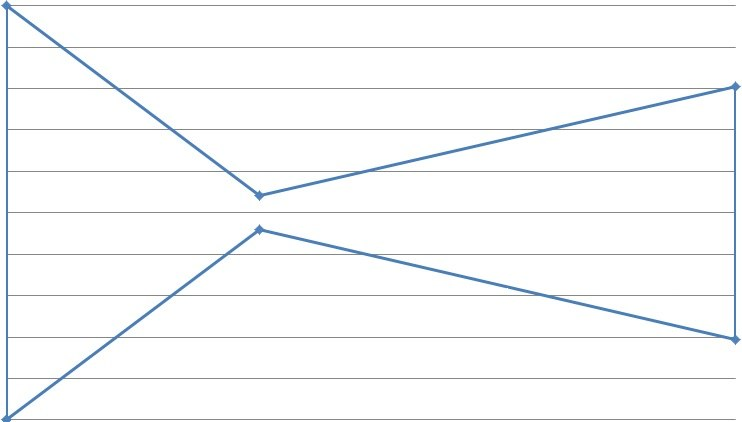
\includegraphics[width=5.7cm, height=3.4cm]{fon.jpg}};
\addplot[mark = none,line width = 0.05 cm, draw =  red ] coordinates {
( -0.059703 , 3199.982829 )
( -0.047762 , 3199.962341 )
( -0.035822 , 3199.899835 )
( -0.023881 , 3199.633135 )
( -0.011941 , 3197.450600 )
( 0.000000 , 2883.073201 )
( 0.023030 , 3151.904598 )
( 0.046060 , 3181.024962 )
( 0.069091 , 3190.820918 )
( 0.092121 , 3194.993353 )
( 0.115151 , 3197.032668 )
( 0.138181 , 3198.128859 )
( 0.161211 , 3198.761568 )
( 0.184241 , 3199.147725 )
( 0.207272 , 3199.394303 )
( 0.230302 , 3199.557758 )
( 0.253332 , 3199.669582 )
( 0.276362 , 3199.748179 )
( 0.299392 , 3199.804726 )
( 0.322423 , 3199.846253 )
( 0.345453 , 3199.877302 )
};
\end{axis}
\end{tikzpicture}
\begin{flushright}
\textit{ Pic. $N^o 15$: STemperature curve projected to the profile nozzle } \\
\end{flushright}
\newpage
\begin{flushright}
\begin{scriptsize}
\textit{160700.65   Проектирование авиационных и ракетных двигателей\\
 Информационные технологии в АКТ: Лабораторный практикум} \\
\end{scriptsize}
\end{flushright}
\begin{tikzpicture}
\begin{axis} [
legend pos = outer north east,
height = 0.19\paperheight,
width = 0.4\paperwidth ]
\legend{  v };
\node[anchor=south west,inner sep=0] at (0,0) {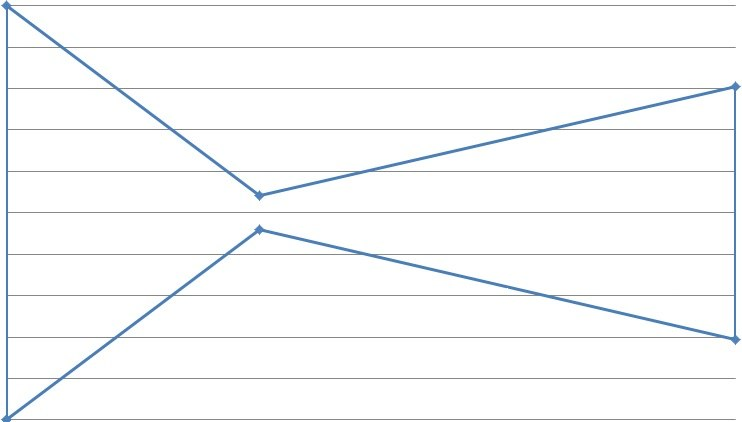
\includegraphics[width=5.7cm, height=3.4cm]{fon.jpg}};
\addplot[mark = none,line width = 0.05 cm, draw =  red ] coordinates {
( -0.059703 , 6.824127 )
( -0.047762 , 10.106071 )
( -0.035822 , 16.481898 )
( -0.023881 , 31.542967 )
( -0.011941 , 83.151114 )
( 0.000000 , 927.104324 )
( 0.023030 , 361.161046 )
( 0.046060 , 226.850874 )
( 0.069091 , 157.778838 )
( 0.092121 , 116.525939 )
( 0.115151 , 89.708209 )
( 0.138181 , 71.236464 )
( 0.161211 , 57.954241 )
( 0.184241 , 48.077187 )
( 0.207272 , 40.530025 )
( 0.230302 , 34.632107 )
( 0.253332 , 29.935098 )
( 0.276362 , 26.133349 )
( 0.299392 , 23.012874 )
( 0.322423 , 20.419854 )
( 0.345453 , 18.241776 )
};
\end{axis}
\end{tikzpicture}
\begin{flushright}
\textit{ Pic. $N^o 16$: Schedule change the speed of the combustion products in the projected nozzle profile } \\
\end{flushright}
\end{document}